\documentclass[a4paper,12pt]{letter}

\usepackage{tikz}
\usepackage{amsmath}
\usepackage{amssymb}
\usepackage{nopageno}
\usepackage{amsmath}
%\usepackage{enumitem}
% \usepackage{mathtools}
%\usepackage{eqnarray,amsmath}
\usepackage[a4paper, total={7.5in, 11.25in}]{geometry}
%\usepackage[margin=2.5cm]{geometry}
\usepackage[utf8]{inputenc}
\usepackage[T1]{fontenc}
\usepackage{lmodern}
%\usepackage{amsmath, amssymb}
\usepackage{setspace}
\setstretch{1.2}
\usepackage{pgfplots}
\pgfplotsset{compat=1.18}

\usetikzlibrary{calc,3d,decorations.pathmorphing,decorations.pathreplacing,decorations.markings,snakes,arrows.meta,calc,patterns}
\tikzset{snake it/.style={decorate, decoration=snake}}

\begin{document}

\begin{center}
 (KTXFI1EBNF) Physics I.  Homework No.~5\\ \smallskip
May~26,~2026
 \end{center}

\begin{enumerate}

\item The wave shown in the figure was generated by a $50\,\mathrm{Hz}$ resonator. Determine:
\begin{enumerate}
\item[a)] amplitude of the wave
\item[b)] frequency of the wave
\item[c)] wavelength of the wave
\item[d)] propagation speed of the wave
\item[e)] period of the wave
\end{enumerate}

\begin{center}
\vskip -30 pt
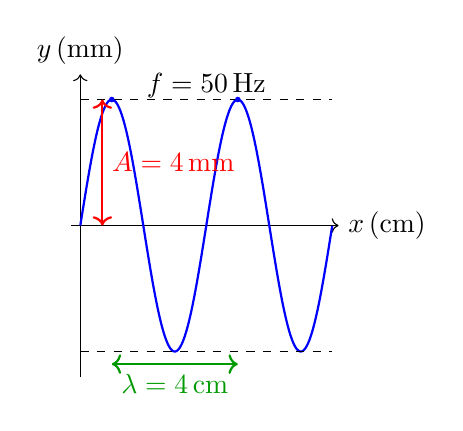
\begin{tikzpicture}[scale=0.4]
\draw[->] (-0.3,0) -- (8.2,0) node[right] {$x\,(\mathrm{cm})$};
\draw[->] (0,-4.8) -- (0,4.8) node[above] {$y\,(\mathrm{mm})$};

\draw[thick,blue,domain=0:8,samples=300] plot(\x,{4*sin(90*\x)});

\draw[dashed] (0,4) -- (8,4);
\draw[dashed] (0,-4) -- (8,-4);

\draw[<->,red,thick] (0.7,0) -- (0.7,4);
\node[red,right] at (0.7,2) {$A=4\,\mathrm{mm}$};

\draw[<->,green!60!black,thick] (1, -4.4) -- (5,-4.4);
\node[green!60!black,below] at (3,-4.4) {$\lambda=4\,\mathrm{cm}$};

\filldraw[blue] (1,4) circle (2pt);
\filldraw[blue] (5,4) circle (2pt);

\node at (4,4.45) {$f=50\,\mathrm{Hz}$};

\end{tikzpicture}
\end{center}
  
% ----------------------------------------------------------------------------------------------------------------------------------------

\item A wave propagating along a string can be defined as follows (with x in meters, t in seconds): $y(x,t)=0.03\,\mathrm{m}\sin(50\,\mathrm{s^{-1}}t-5\,\mathrm{m^{-1}}\,x).$ Determine the:
\begin{enumerate}
\item[a)] amplitude
\item[b)] frequency
\item[c)] wavelength
\item[d)] speed
\end{enumerate}

% ----------------------------------------------------------------------------------------------------------------------------------------

\item Determine the amplitude, frequency, and wavelength of the wave shown in the figure below, if the propagation speed of the wave is 340\,m/s. Write a solution for the wave if at t=1\,s the wave appears as shown in the figure.

\begin{center}
\vskip -20 pt
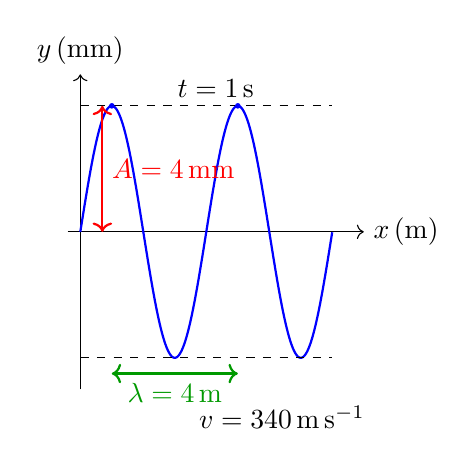
\begin{tikzpicture}[scale=0.4]
\draw[->] (-0.4,0) -- (9,0) node[right] {$x\,(\mathrm{m})$};
\draw[->] (0,-5) -- (0,5) node[above] {$y\,(\mathrm{mm})$};

\draw[thick,blue,domain=0:8,samples=300] plot(\x,{4*sin(90*\x)});

\draw[dashed] (0,4) -- (8,4);
\draw[dashed] (0,-4) -- (8,-4);

\draw[<->,red,thick] (0.7,0) -- (0.7,4);
\node[red,right] at (0.7,2) {$A=4\,\mathrm{mm}$};

\draw[<->,green!60!black,thick] (1,-4.5) -- (5,-4.5);
\node[green!60!black,below] at (3,-4.5) {$\lambda=4\,\mathrm{m}$};

\filldraw[blue] (1,4) circle (2pt);
\filldraw[blue] (5,4) circle (2pt);

\node at (4.3,4.55) {$t=1\,\mathrm{s}$};
\node at (6.4,-5.9) {$v=340\,\mathrm{m\,s^{-1}}$};
\end{tikzpicture}
\end{center}

% ----------------------------------------------------------------------------------------------------------------------------------------

\item For a wave propagating along a string with a frequency of 10\,Hz, $\lambda$ = 80\,cm, A$=$3\,mm, write the solution in SI units.

  
% ----------------------------------------------------------------------------------------------------------------------------------------

\item A wave solution is given by $y = 0.3 \sin(15x - 600t)\,mm$, where x is in meters and t is in seconds. For the transverse wave at x=30\,cm, determine:
\begin{enumerate}
\item[a)] its speed
\item[b)] its acceleration
\item[c)] What is the displacement of the point at t=4\,s?
\end{enumerate}

  
% ----------------------------------------------------------------------------------------------------------------------------------------

\end{enumerate}

\bigskip

\rightline{Dr.~Gabor~FACSKO}
\rightline{\textit{facsko.gabor@uni-obuda.hu}}

\vfill

\end{document}
